\section{Appendix}\label{sec:Appendix}

As mentioned in the discussion above, table \ref{tab:accuracy} seemed to indicate that the models were highly overfitted to the training data, which resulted in terrible test performance in setting 2. In order to deal with this problem, we experimented with using trees with fewer splits. We achieved a significant increase in accuracy score by doing this, as shown in table \ref{tab:accuracy2}. By reducing the tree depth to 3 for the decision tree, bagging and random forest, the test accuracies were raised to $40.3\%$, $40.2\%$ and $45.1\%$ for the respective methods. Figure \ref{fig:decisiontree} shows a graphical overview of the decision tree with a maximum depth of 3, and one thing to note is that only 5 of the 7 classes are represented by the leaf nodes, which is something that also should be considered when creating biased tree models with shallow depths.

The boosting methods were also improved by reducing both the max depth, the number of estimators and the learning rate, and XGBoost gave the best accuracy score, $60.5\%$, with a max depth of only $1$. The resulting confusion matrix based on the XGBoost model is shown in figure \ref{fig:xgboost_confusion_matrix}. It is clear that the results have improved greatly for setting 2, but it is still far from usable in terms of separating the seven activities based on the dataset. 

\begin{figure}
    \centering
    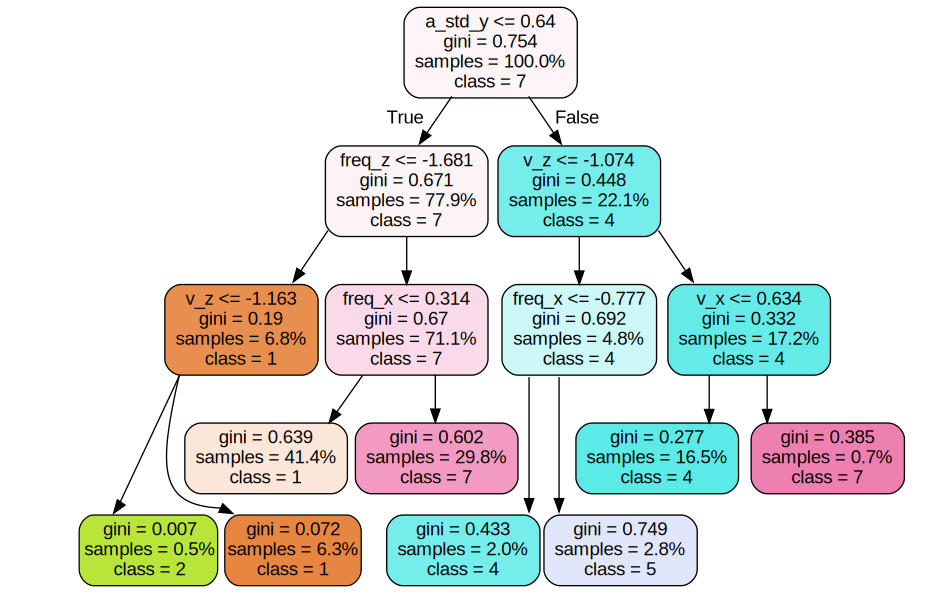
\includegraphics[scale=0.58]{Figures/activity_tree.pdf}
    \caption{Decision tree for setting 2, and an accuracy of $40.3\%$.}
    \label{fig:decisiontree}
\end{figure}

\begin{table}[]
\caption{Accuracy of classifiers on setting 2, when using a shallow depth in order to reduce overfitting.}
\begin{tabular}{|l|c|c|c|c|}
\hline
Classifier & Estimators & Max depth & Learning rate & Accuracy \\
\hline
Decision tree      & 200  & 3 & N/A  & 40.3   \\ \hline
Bagging            & 200  & 3 & N/A  & 40.2  \\ \hline
Random forest      & 200  & 3 & N/A  & 45.1  \\ \hline
AdaBoost           & 50  & 1 & 0.01  & 35.3  \\ \hline
Gradient boosting  & 50  & 1 & 0.01  & 43.6  \\ \hline
XGBoost            & 50  & 1 & 0.01  & 60.5  \\ \hline
\end{tabular}'
\label{tab:accuracy2}
\end{table}

\begin{figure}
    \centering
    \includegraphics[scale=0.8]{Figures/20191206-125914-confusionmatrix.pdf}
    \caption{Confusion matrix using XGBoost, with parameters as specified in table \ref{tab:accuracy2}, and an accuracy score of $60.5\%$.}
    \label{fig:xgboost_confusion_matrix}
\end{figure}

Another possibility is to simplify the targets, and check whether the learning algorithms perform better when dealing with activity categories, instead of the relatively specific activities we had in the original dataset. In order to investigate this, we combined the target in the following way:

\begin{itemize}
    \item \textbf{1. Working at computer} (unchanged class 1).
    \item \textbf{2. Standing.} Combined class 3 ("standing") and 7 ("talking while standing").
    \item \textbf{3. Walking.} Combined class 4 ("walking") and 6 ("walking and talking with someone").
    \item \textbf{4. Going up/down stairs} (unchanged class 5).
    \item Class 2 ("standing up, walking and going up/down stairs") was removed from the dataset, due to its complex nature.
\end{itemize}

With this simplified dataset, we created a new model using XGBoost, with 50 estimators, max depth of 3, and a learning rate of $0.01$. The resulting accuracy score was $65.5\%$, and the confusion matrix is shown in figure \ref{fig:xgboost_confusion_matrix_simplified}. As we can see, this model is performing better, but still confuses some activity categories. The most notable confusion happens between class 3 and 4 of the simplified targets, "walking" and "going up/down stairs", which intuitively is reasonable, since these are similar activities that both involve walking.


\begin{figure}
    \centering
    \includegraphics[scale=0.8]{Figures/20191206-182459-confusionmatrix.pdf}
    \caption{Confusion matrix using XGBoost on a simplified dataset, giving an accuracy score of $65.5\%$. Number of estimators was 50, max depth 3, and the learning rate $0.01$.}
    \label{fig:xgboost_confusion_matrix_simplified}
\end{figure}
